The following mockups represent the final look of the application in great detail. They are based on the sketches provided in the RASD. Material design principles were used as inspiration in the design process.

{
\setlength{\fboxsep}{0pt}
\begin{figure}[H]
\centering
\begin{minipage}{.4\textwidth}
    \centering
    \fbox{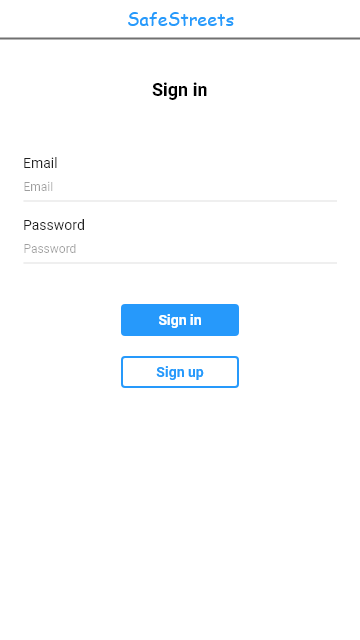
\includegraphics[width=.8\textwidth]{Images/ui/sign-in.png}}
    \caption{\label{fig:mockup-sign-in}Mockup - Sign in.}
\end{minipage}
\begin{minipage}{.4\textwidth}
    \centering
    \fbox{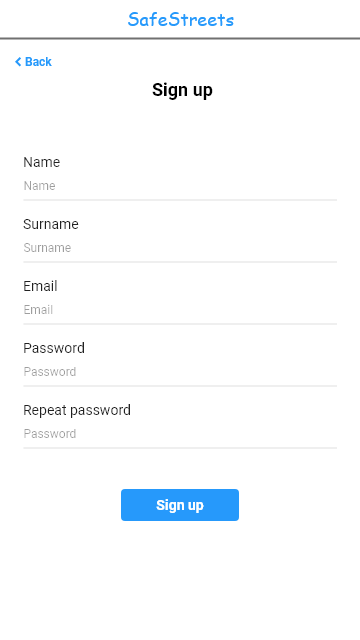
\includegraphics[width=.8\textwidth]{Images/ui/sign-up.png}}
    \caption{\label{fig:mockup-sign-up}Mockup - Sign up.}
\end{minipage}
\end{figure}

\begin{figure}[H]
\centering
\begin{minipage}{.4\textwidth}
    \centering
    \fbox{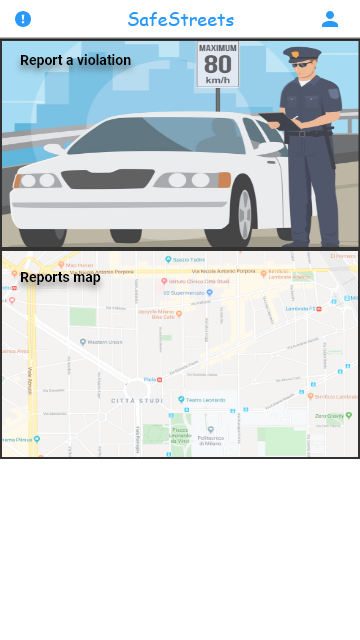
\includegraphics[width=.8\textwidth]{Images/ui/home.png}}
    \caption{\label{fig:mockup-home}Mockup - Home.}
\end{minipage}
\begin{minipage}{.4\textwidth}
    \centering
    \fbox{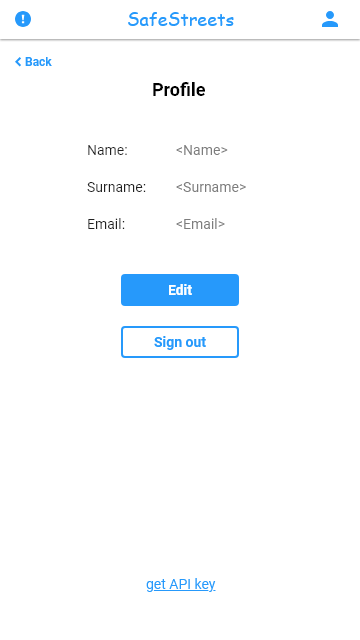
\includegraphics[width=.8\textwidth]{Images/ui/profile.png}}
    \caption{\label{fig:mockup-profile}Mockup - Profile.}
\end{minipage}
\end{figure}

\begin{figure}[H]
\centering
\begin{minipage}{.4\textwidth}
    \centering
    \fbox{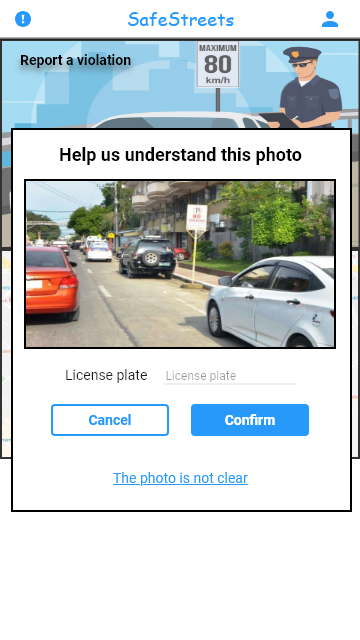
\includegraphics[width=.8\textwidth]{Images/ui/photo-review.png}}
    \caption{\label{fig:mockup-photo-review}Mockup - Photo review.}
\end{minipage}
\begin{minipage}{.4\textwidth}
    \centering
    \fbox{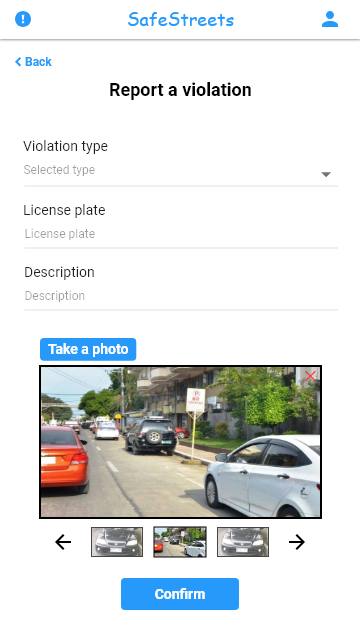
\includegraphics[width=.8\textwidth]{Images/ui/report-violation.png}}
    \caption{\label{fig:mockup-report-violation}Mockup - Report violation.}
\end{minipage}
\end{figure}

\begin{figure}[H]
\centering
\begin{minipage}{.4\textwidth}
    \centering
    \fbox{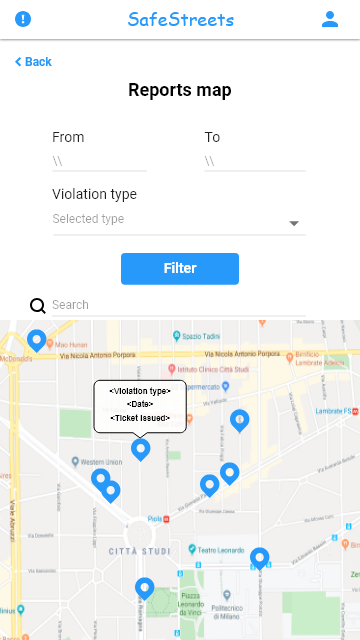
\includegraphics[width=.8\textwidth]{Images/ui/reports-map.png}}
    \caption{\label{fig:mockup-reports-map}Mockup - Reports map.}
\end{minipage}
\end{figure}
}

Here is a description of each screen and its functionalities:\\

\begin{itemize}
\item
Sign in: Form for the user to access the system.
\item
Sign up: Form for the user to register in the system.
\item
Home: Main screen of the application, from here the user can access every functionality.
\item
Profile: Shows the user's personal information and allows them to modify it. Also allows the user to request an API key and sign out.
\item
Photo review: The user is required to input the license plate being shown in the photo, or specify that is not clear enough.
\item
Report violation: Form to submit a report violation. Includes a preview of the photos taken where they can be discarded.
\item
Reports map: A map with the reports is shown, the user is capable of filtering the results by date, type and location. When pressing on a report, a popup with details appears.
\end{itemize}

The flow of the application can be seen in [figure n], where the arrows represent a transition between two screens. As it can be appreciated, every functionality can be accessed from the home screen.

\begin{figure}[H]
\centering
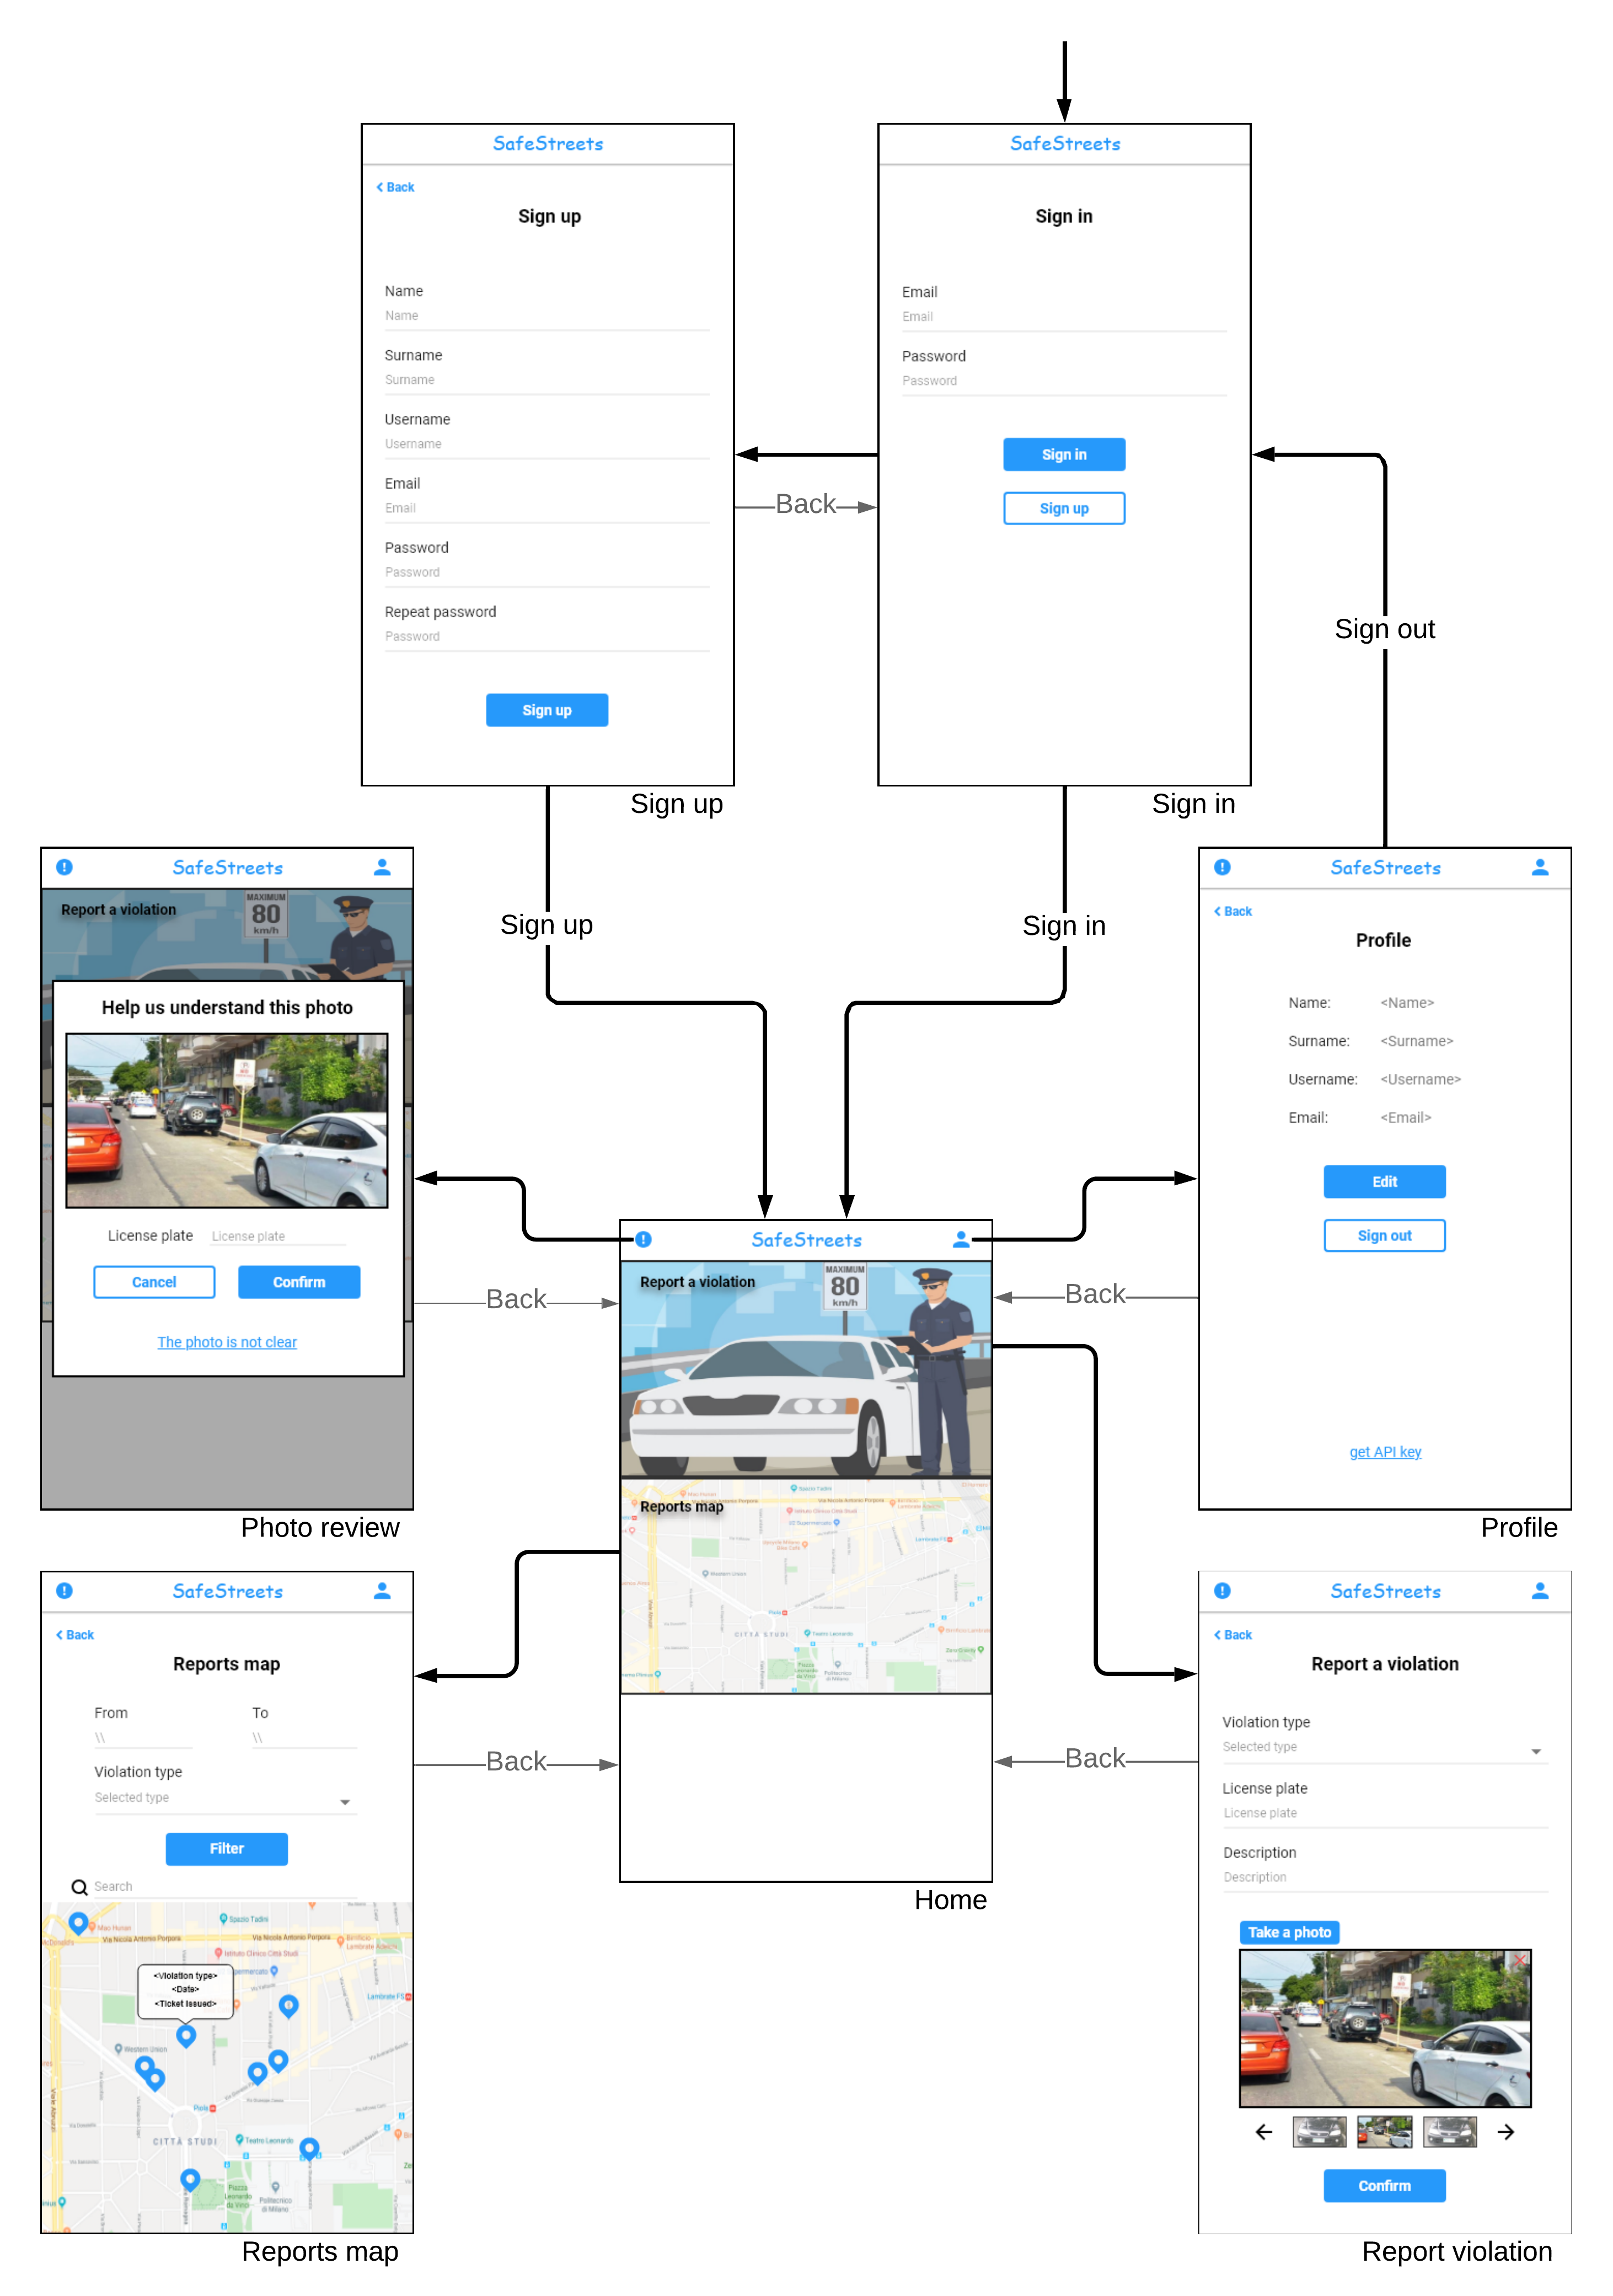
\includegraphics[width=\textwidth]{Images/mobile-flow.png}
\caption{\label{fig:api-usage}Mobile application flow.}
\end{figure}